% SPI integrationstest
\label{section:spi_integrationstest}
%tekst

I det følgende testes SPI-kommunikationen. Alle kommandoer testes for sig og dokumenteres herunder ved logik analyse billeder samt tabeller der er udarbejdet af eksporterede .txt filer fra Salae Logic \footnote{Salae Logic er softwaren der benyttes til USB logic analyser. Det er herfra at analysebilleder samt data til tabellerne er fra}. 


% Aktiver
\subsubsection*{Aktiver}

Aktiver testes med et testobjekt

\begin{lstlisting}[language=C]
int main(void){
	SPI_api test;
	test.activate(1); // 1 er et dummy enhedsnummer
}
\end{lstlisting}

\begin{figure}[H]
\centering
{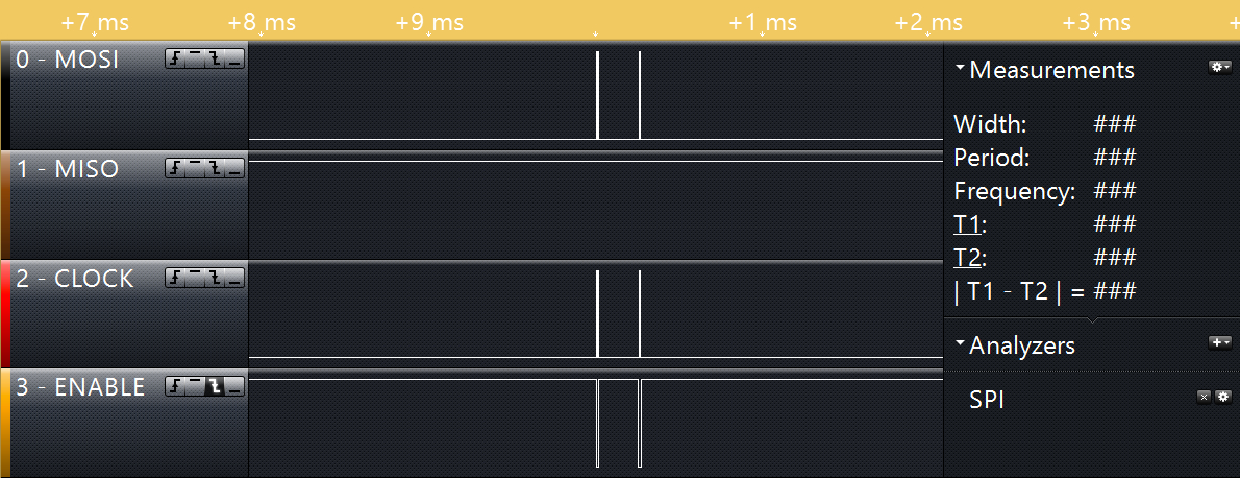
\includegraphics[width=0.90\textwidth]{filer/integrationstest/billeder/spi_activate}}
\caption{Analysebillede for kommandoen aktiver fra Logic-Analyzer}
\label{lab:scop_activate}
\end{figure}

Tabel \ref{table:scop_activate} viser dataoverførelsen. Som det ses har kun MOSI betydning for aktiver, da aktiver er en write metode. 

\begin{table}[H]
	\caption{Analysedata eksporteret til tabel}
	\centering
	\begin{tabular}{|l|c|c|}
		\hline 
		\textbf{Char nr} & \textbf{0} & \textbf{1} \\ 		
		\hline 
		\textbf{MOSI} & '\verb+A+' & '\verb+C+' \\ 
		\hline 
		\textbf{MISO} & '\verb+255+' & '\verb+255+' \\ 
		\hline 
	\end{tabular} 
	\label{table:scop_activate}
\end{table}


% Deaktiver
\subsubsection*{Deaktiver}
Deaktiver testes med et testobjekt

\begin{lstlisting}[language=C]
int main(void){
	SPI_api test;
	test.deactivate(1); // 1 er et dummy enhedsnummer
}
\end{lstlisting}

\begin{figure}[H]
\centering
{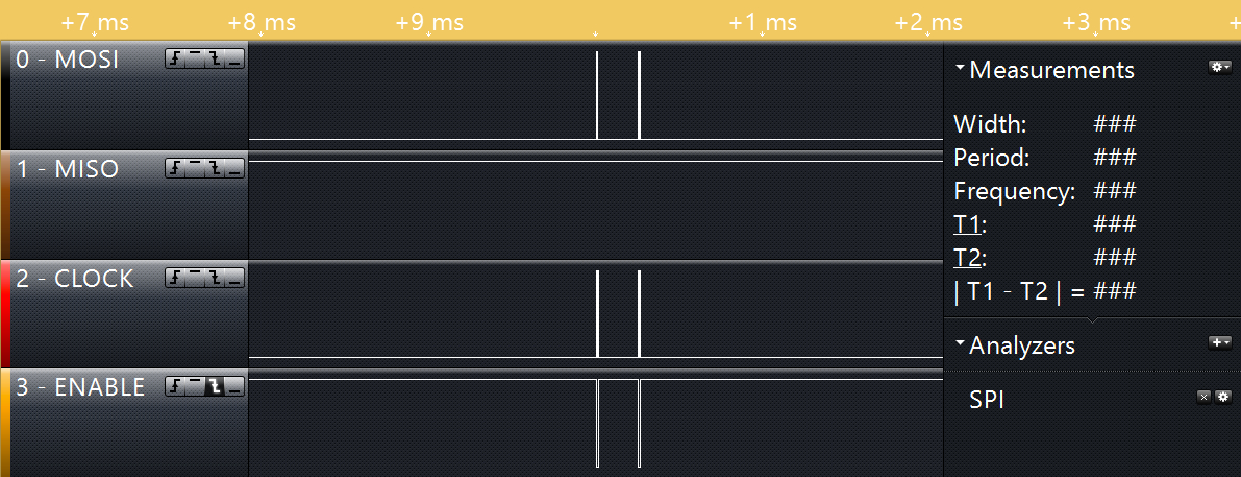
\includegraphics[width=0.90\textwidth]{filer/integrationstest/billeder/spi_deactivate}}
\caption{Analysebillede for kommandoen deaktiver fra Logic-Analyzer}
\label{lab:scop_deactivate}
\end{figure}

Tabel \ref{table:scop_deactivate} viser dataoverførelsen. Som det ses har kun MOSI betydning for deaktiver, da deaktiver er en write metode. 

\begin{table}[h]
	\caption{Analysedata eksporteret til tabel}
	\centering
	\begin{tabular}{|l|c|c|}
		\hline 
		\textbf{Char nr} & \textbf{0} & \textbf{1} \\ 		
		\hline 
		\textbf{MOSI} & '\verb+D+' & '\verb+C+' \\ 
		\hline 
		\textbf{MISO} & '\verb+255+' & '\verb+255+' \\ 
		\hline 
	\end{tabular} 
	\label{table:scop_deactivate}
\end{table}


% Config
\subsubsection*{Config}
Config testes med 2 test-floats der sendes med config metoden.

\begin{lstlisting}[language=C]
int main(void){
	float tempTest = 100.1;
	float humiTest = 48;
	SPI_api test;
	
	test.config(1, tempTest, humiTest); // 1 er et dummy enhedsnummer
}
\end{lstlisting}



\begin{figure}[H]
\centering
{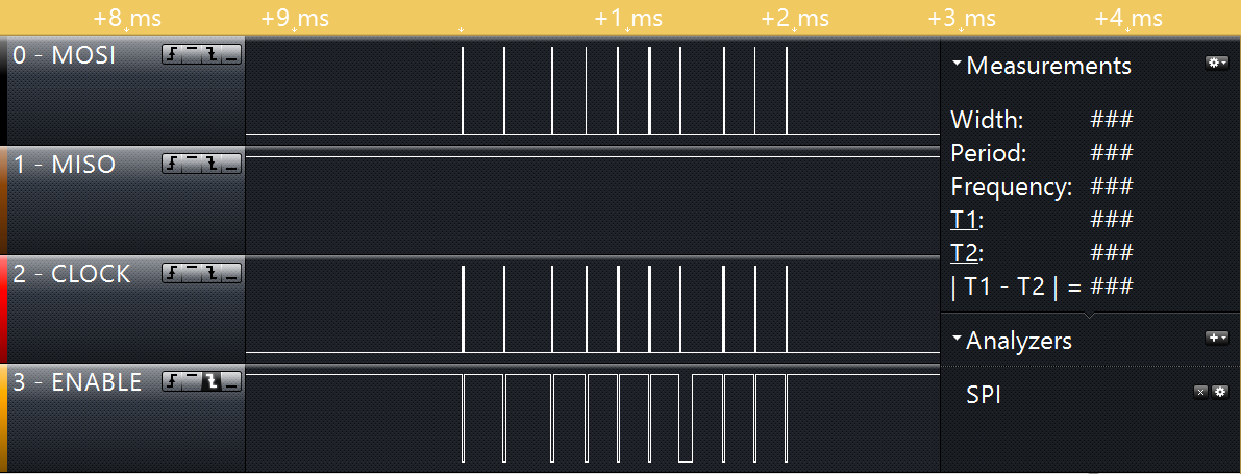
\includegraphics[width=0.90\textwidth]{filer/integrationstest/billeder/spi_config}}
\caption{Analysebillede for kommandoen config fra Logic-Analyzer}
\label{lab:scop_config}
\end{figure}

Tabel \ref{table:scop_config} viser dataoverførelsen. Som det ses har kun MOSI betydning for config, da config er en write metode. 

\begin{table}[H]
	\caption{Analysedata eksporteret til tabel}
	\centering
	\begin{tabular}{|l|c|c|c|c|c|c|c|c|c|c|}
		\hline 
		\textbf{Char nr} & \textbf{0} & \textbf{1} & \textbf{2} & \textbf{3} & \textbf{4} & \textbf{5} 
						 & \textbf{6} & \textbf{7} & \textbf{8} & \textbf{9}\\ 		
		\hline 
		\textbf{MOSI} & '\verb+P+' & '\verb+1+' & '\verb+0+' & '\verb+0+' & '\verb+.+' & '\verb+1+' 
						& '\verb+0+' & '\verb+4+' & '\verb+8+' & '\verb+C+' \\ 
		\hline 
		\textbf{MISO} & '\verb+255+' & '\verb+255+' & '\verb+255+' & '\verb+255+' & '\verb+255+' & '\verb+255+' 
						& '\verb+255+' & '\verb+255+' & '\verb+255+' & '\verb+255+' \\ 
		\hline 
	\end{tabular} 
	\label{table:scop_config}
\end{table}


% Verificer
\subsubsection*{Verificer}
Verify testes med et test objekt og der sendes et 1-tal af sted til sammenligning med Enhedens enhedsnummer.

\begin{lstlisting}[language=C]
int main(void){
	SPI_api test;	
	test.verify(1);
}
\end{lstlisting}

\begin{figure}[H]
\centering
{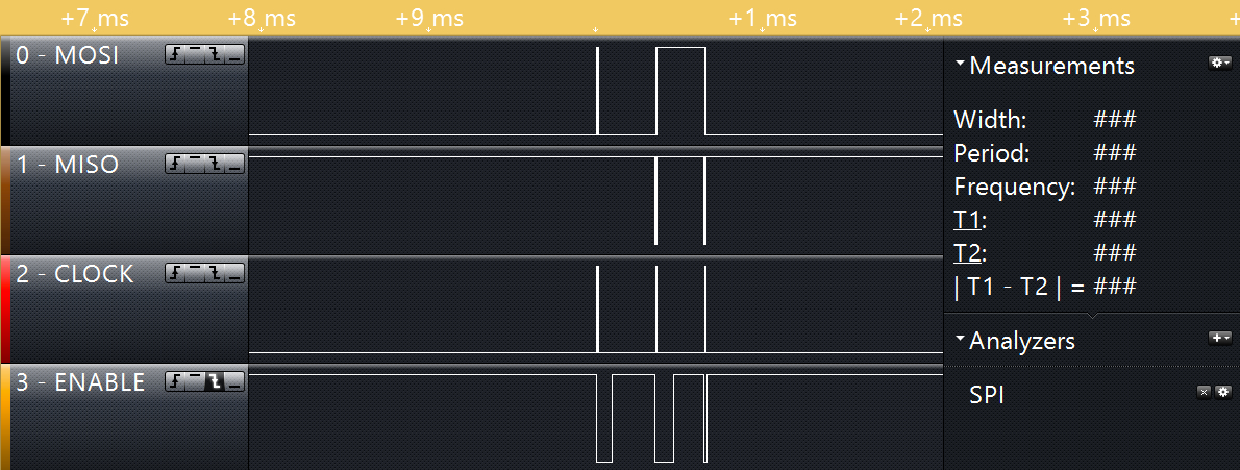
\includegraphics[width=0.90\textwidth]{filer/integrationstest/billeder/spi_verify}}
\caption{Analysebillede for kommandoen verificer fra Logic-Analyzer}
\label{lab:scop_verify}
\end{figure}

Tabel \ref{table:scop_verify} viser dataoverførelsen. Som det ses overføres der data på både MOSI og MISO linjen. Det sker da verificer er en read-metode. Testen her er udført med tilkoblet Enhed. Hvis enheden kobles fra og der ikke modtages et matchende enhedsnummer, returneres en fejlkode i programmet. 
 

\begin{table}[H]
	\caption{Analysedata eksporteret til tabel}
	\centering
	\begin{tabular}{|l|c|c|c|}
		\hline 
		\textbf{Char nr} & \textbf{0} & \textbf{1} & \textbf{2}\\ 		
		\hline 
		\textbf{MOSI} & '\verb+V+' & '\verb+R+'  & '\verb+C+'\\ 
		\hline 
		\textbf{MISO} & '\verb+255+' & '\verb+1+' & '\verb+0+' \\ 
		\hline 
	\end{tabular} 
	\label{table:scop_verify}
\end{table}


% Log

\subsubsection*{Log}
Getlog metoden testes vha. et testobjekt og med en testbuffer i form af et char array på Enheden. Der er også sat en for-løkke ind til at udskrive strengene i vektoren.

\begin{lstlisting}[language=C]
char testGetLog[] = "DTTT.TFFFVBEXXX";
\end{lstlisting}

\begin{lstlisting}[language=C++]
	int testUnits = 1;
	vector<string> test_data;
	SPI_api test;

	test.getLog(test_data, &testUnits, 1);
	
	for(unsigned int i = 0 ; i < test_data.size() ; i++)
		std::cout << "test_data[" << i << "]: " << test_data[i] << endl;
\end{lstlisting}

\begin{figure}[H]
\centering
{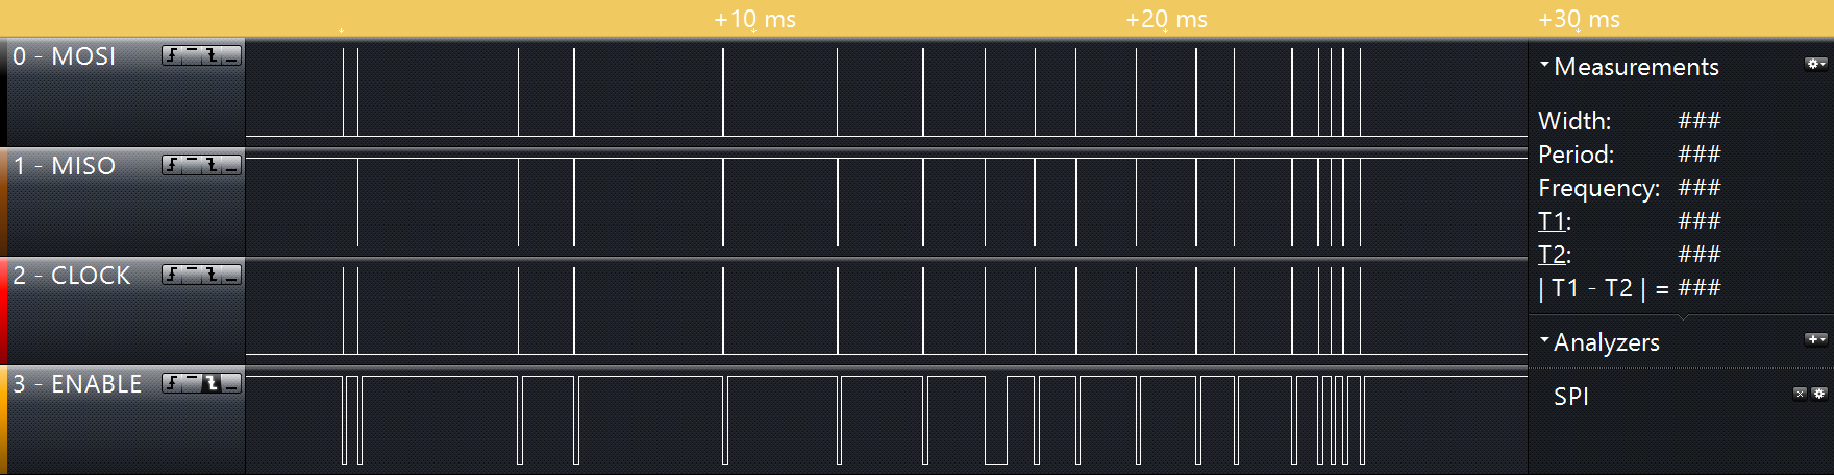
\includegraphics[width=0.90\textwidth]{filer/integrationstest/billeder/spi_getlog_and_error}}
\caption{Analysebillede for kommandoen getLog fra Logic-Analyzer}
\label{lab:scop_getlog}
\end{figure}

Tabel \ref{table:scop_getlog1} og \ref{table:scop_getlog2} viser dataoverførelsen. 

\begin{table}[H]
	\caption{Analyse data eksporteret til tabel del 1}
	\centering
	\begin{tabular}{|l|c|c|c|c|c|c|c|c|c|c|}
		\hline 
		\textbf{Char nr} & \textbf{0} & \textbf{1} & \textbf{2} & \textbf{3} & \textbf{4} & \textbf{5} 
						 & \textbf{6} & \textbf{7} & \textbf{8} & \textbf{9}\\ 		
		\hline 
		\textbf{MOSI} & '\verb+L+' & '\verb+R+' & '\verb+R+' & '\verb+R+' & '\verb+R+' & '\verb+R+' 
						& '\verb+R+' & '\verb+R+' & '\verb+R+' & '\verb+R+'\\ 
		\hline 
		\textbf{MISO} & '\verb+255+' & '\verb+16+' & '\verb+D+' & '\verb+T+' & '\verb+T+' & '\verb+T+' 
						& '\verb+.+' & '\verb+T+' & '\verb+F+' & '\verb+F+'\\
						 
		\hline 
	\end{tabular} 
	\label{table:scop_getlog1}
\end{table}


\begin{table}[H]
	\caption{Analysedata eksporteret til tabel del 2}
	\centering
	\begin{tabular}{|l|c|c|c|c|c|c|c|c|}
		\hline 
		\textbf{Char nr} & \textbf{10} & \textbf{11} & \textbf{12} & \textbf{13}
						& \textbf{14} & \textbf{15} & \textbf{16} & \textbf{17}\\ 		
		\hline 
		\textbf{MOSI} 	& '\verb+R+' & '\verb+R+' & '\verb+R+' & '\verb+R+'
						& '\verb+R+' & '\verb+R+' & '\verb+R+' & '\verb+R+' \\ 
		\hline 
		\textbf{MISO}	& '\verb+F+' & '\verb+V+' & '\verb+B+' & '\verb+E+'
						& '\verb+X+' & '\verb+X+' & '\verb+X+' & '\verb+0+'\\
						 
		\hline 
	\end{tabular} 
	\label{table:scop_getlog2}
\end{table}

Outputtet fra udskriften af \verb+test_data+ vektoren:

\verb+test_data[0]: DTTT.TFFFVB+ \newline
\verb+test_data[1]: EXXX+

Helt som forventet.

Der er ligeledes testet med et mere komplekst char array med flere data og error strenge. Disse læses også som de skal. 

\subsubsection*{Begrænsninger}

Ovenstående modultest er udført med et 7 cm langt fladkabel til forbindelsen mellem Master og Enhed. Der er testet med et 22 cm langt fladkabel, her var der en fejlrate på mere end 10 \%. Ydermere er det nødvendigt at være opmærksom på ikke at lade nogle kabler krydse fladkablet, da dette giver støj og vil medføre fejl. Der er ikke oplevet fejl ved at benytte fladkablet på 7 cm, så længe støjkilder holdes på afstand.   